\chapter{Návrh riešenia}
\label{kapitola4}
V tejto kapitole sa čitateľ zoznámi s návrhom celej aplikácie. V prvej sekcii sú rozobrané prípady použitia aplikácie. Ďalej sa čitateľ dočíta o návrhu architektúry systému, o návrhu užívateľského rozhrania, o návrhu databázy a na záver o návrhu serverovej aj klientskej časti aplikácie.

\section{Použitie aplikácie}
\label{pouzitie}
Pri príchode na webovú stránku sa užívateľ ocitne na autentifikačnej stránke, kde sa musí prihlásiť, alebo zaregistrovať, aby mohol postúpiť ďalej.

Po úspešnom prihlásení užívateľ je presmerovaný na domovskú stránku. Na domovskej stránke má prístup k zoznamu vlastných prezentácií, ktoré už vytvoril. Vie si tu vytvoriť novú prezentáciu kliknutím na tlačítko \texttt{Create New}, alebo sa odhlásiť tlačítkom \texttt{Logout}. Zoznam obsahuje kartičky jednotlivých prezentácií so stručným popisom informácií. Kartička obsahuje tlačítko \texttt{Delete} pre odstránenie celej prezentácie. Kliknutím na kartičku sa zobrazí detailný popis prezentácie. V detaily má užívateľ prístup k vytvoreným verziám a popisom k nim. Nachádza sa tu náhľad do stránok jednotlivých verzií pre uľahčenie voľby správnej verzie. Užívateľ si vie zobraziť prezentáciu v prezentačnom móde cez tlačítko \texttt{View}, upraviť verziu cez tlačítko \texttt{Edit} a odstrániť verziu tlačítkom \texttt{Delete v\_}.

Pri vytváraní novej prezentácie, alebo upravovaní už existujúcej nás aplikácie presmeruje na stránku editora. Editor obsahuje mnoho užitočných nástrojov pre zjednodušenie tvorby pomocou jazyka Markdown, ako napríklad typografické nástroje, vloženie zoznamov, tabuliek, obrázkov, odkazov a častí zdrojového kódu. Veľkou výhodou je výskyt náhľadu v editore, kde je hneď vidieť sformátovaný obsah stránky. V bočnom paneli má užívateľ možnosť sa vrátiť na domovskú stránku cez tlačítko \texttt{Home}. Po kliknutí na tlačítko \texttt{Save} sa zobrazí panel na uloženie prezentácie. Pri upravovaní prezentácie aplikácia ponúka úpravu názvu a pridanie popisu k verzii. Prezentáciu vie tvorca uložiť pod novou verziou, alebo môže aktualizovať práve upravovanú verziu. Kliknutím na tlačítko \texttt{Preview} sa aplikácia prepne do prezentačného módu. Prepínanie stránok v prezentačnom móde funguje pomocou klávesnicových šípok. 

Tvorca si vie zobraziť panel so stránkami cez tlačítko \texttt{Slides}. Panel obsahuje zoznam jednotlivých stránok prezentácie. Ich poradie môže byť upravené pomocou technológie ťahaj-a-pusti (drag-and-drop). Užívateľ má možnosť prepnutia zoznamu stránok do mriežkového pohľadu(grid view), kde sa dá jednoduchšie orientovať a usporiadať jednotlivé stránky. Aplikácia umožňuje kopírovanie stránok medzi prezentáciami jednoduchým kliknutím na tlačítka \texttt{Kopírovať} a \texttt{Prilepiť}.

\section{Architektúra aplikácie}
\label{architecture}
Aplikácia je rozdelená na dve časti, na klientskú a serverovú. Jedná sa o takzvanú dvojvrstvovú architektúru \texttt{klient-server}. Klientská časť sa nazýva aj ako prezentačná vrstva. Poskytuje interaktivitu užívateľom, má za úlohu zobrazovanie obsahu a údajov získaných zo servera. Zbiera užívateľom zadané dáta cez rôzne vstupy. Tieto dáta môžu byť spracovávané a upravované už na klientovi a sú posielané na server cez protokol HTTP\footnote{Hypertextový prenosový protokol} pomocou knihovne \textit{axios}. Server údaje prijíma a ďalej spracováva. Medzi úlohy serverovej časti patria: prijímanie požiadavkov od klienta, posielanie odpovedí na požiadavky stavovými kódmi a údajmi, zabezpečenie a udržovanie komunikácie cez autentifikáciu a autorizáciu užívateľov, vykonávanie rôznych výpočtov, formátovanie údajov pre databázu, alebo klienta. Klient nekomunikuje priamo s databázou, na to slúži server. Server údaje od klienta upravuje, aby vyhovovali formátu v databáze. Taktiež si vypýta dáta z databázy, ktoré spracováva a posiela klientovi. Grafické znázornenie architektúry pre jednoduchšie pochopenie sa nachádza na obrázku \ref{pic:architektura}.

    \begin{figure}[!hbt]
        \centering
        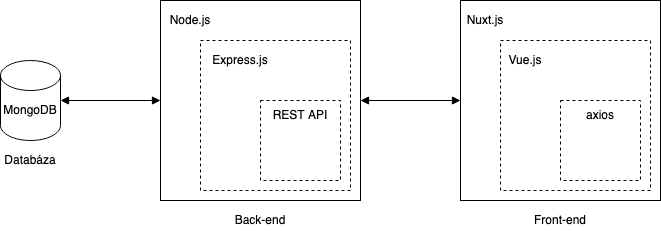
\includegraphics[scale=0.6]{obrazky/architektura.png}
        \caption{Znázornenie architektúry aplikácie.}
        \label{pic:architektura}
    \end{figure}
    
\section{Návrh frontendu}
V aplikácii sa využíva framework Nuxt.js, ktorý je nadstavbou Vue.js. Nuxt.js uľahčuje vývoj jednostránkových aplikácií a poskytuje vývojárom lepší zážitok pri programovaní. 
Aktuálne stabilná verzia Vue.js a Nuxt.js pri začatí projektu je verzia 2, ale v aplikácii sa už využívajú \texttt{composition-api} vlastnosti verzie 3, ktoré je potrebné nainštalovať ako balík cez NPM a pridať medzi moduly Nuxt.js v konfiguračnom súbore.

\subsection{Pohľad aplikácie}
Pohľad v Nuxt.js aplikácii sa skladá z viacerých vrstiev. Najvyššia vrstva je HTML súbor \texttt{App.html}, ktorý je vytvorený automaticky a slúži pre vytvorenie kostry aplikácie. Tento súbor obsahuje všetok obsah, atribúty pre hlavičku a telo HTML dokumentu. 

Nižšia vrstva obsahuje šablónu aplikácie, pomocou ktorej sa zadefinuje rovnaký obsah na viacerých stránkach. Dobrým príkladom pre obsah v šablóne je navbar, ktorý môže byť dostupný na viacerých stránkach aplikácie. 

Pod šablónou sa nachádzajú komponenty jednotlivých stránok aplikácie. Každá stránka je samostatná Vue komponentom, ku ktorým Nuxt.js prideľuje špeciálne atribúty a funkcie. Medzi ne patrí \textbf{useFetch}, funkcia pre asynchrónne sťahovanie dát hneď pri návšteve stránky, naďalej atribút \textbf{auth} vyžadujúci autentifikáciu pre navštívenie stránky, alebo atribút \textbf{layout} určujúci, ktorú šablónu má stránka využívať.

Každá stránka môže mať niekoľko potomkov. Potomok má rovnakú štruktúru ako rodičovská stránka a taktiež obsahuje Nuxtom pridelené atribúty a funkcie. Stránka sa môže skladať z viacerých komponentov, ich výhody už boli v tejto práci zmienené vyššie.

    \begin{figure}[!hbt]
        \centering
        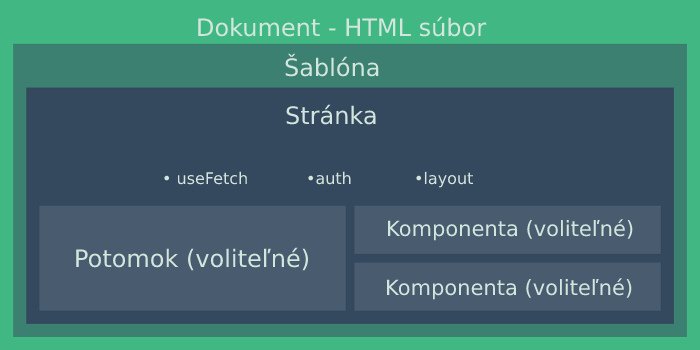
\includegraphics[scale=0.4]{obrazky/nuxt_struktura.png}
        \caption{Kompozícia pohľadu v Nuxt.js.}
        \label{pic:nuxt_strukture}
    \end{figure}


\subsection{Užívateľské rozhranie}
\label{navrhui}
Užívateľské rozhranie je dôležitou súčasťou aplikácie. Je to časť, s ktorou užívateľ pracuje, a preto je dôležité, aby orientácia na nej bola čím jednoduchšia a prehľadnejšia. Cieľom bolo vytvoriť minimalistické rozhranie, na ktorom sa ľahko nájdu potrebné ovládacie prvky.

Prototyp rozhrania bol vytvorený pomocou návrhového programu Adobe XD. Prvý návrh domovskej stránky a editora je vidieť na obrázku \ref{pic:prototyp_domovska_stranka} a \ref{pic:prototyp_editor}. Odvtedy aplikácia prešla viacerými prestavbami a dizajn sa výrazne zmenil.

\begin{figure}[!hbt]
\centering
\begin{minipage}{.5\textwidth}
  \centering
  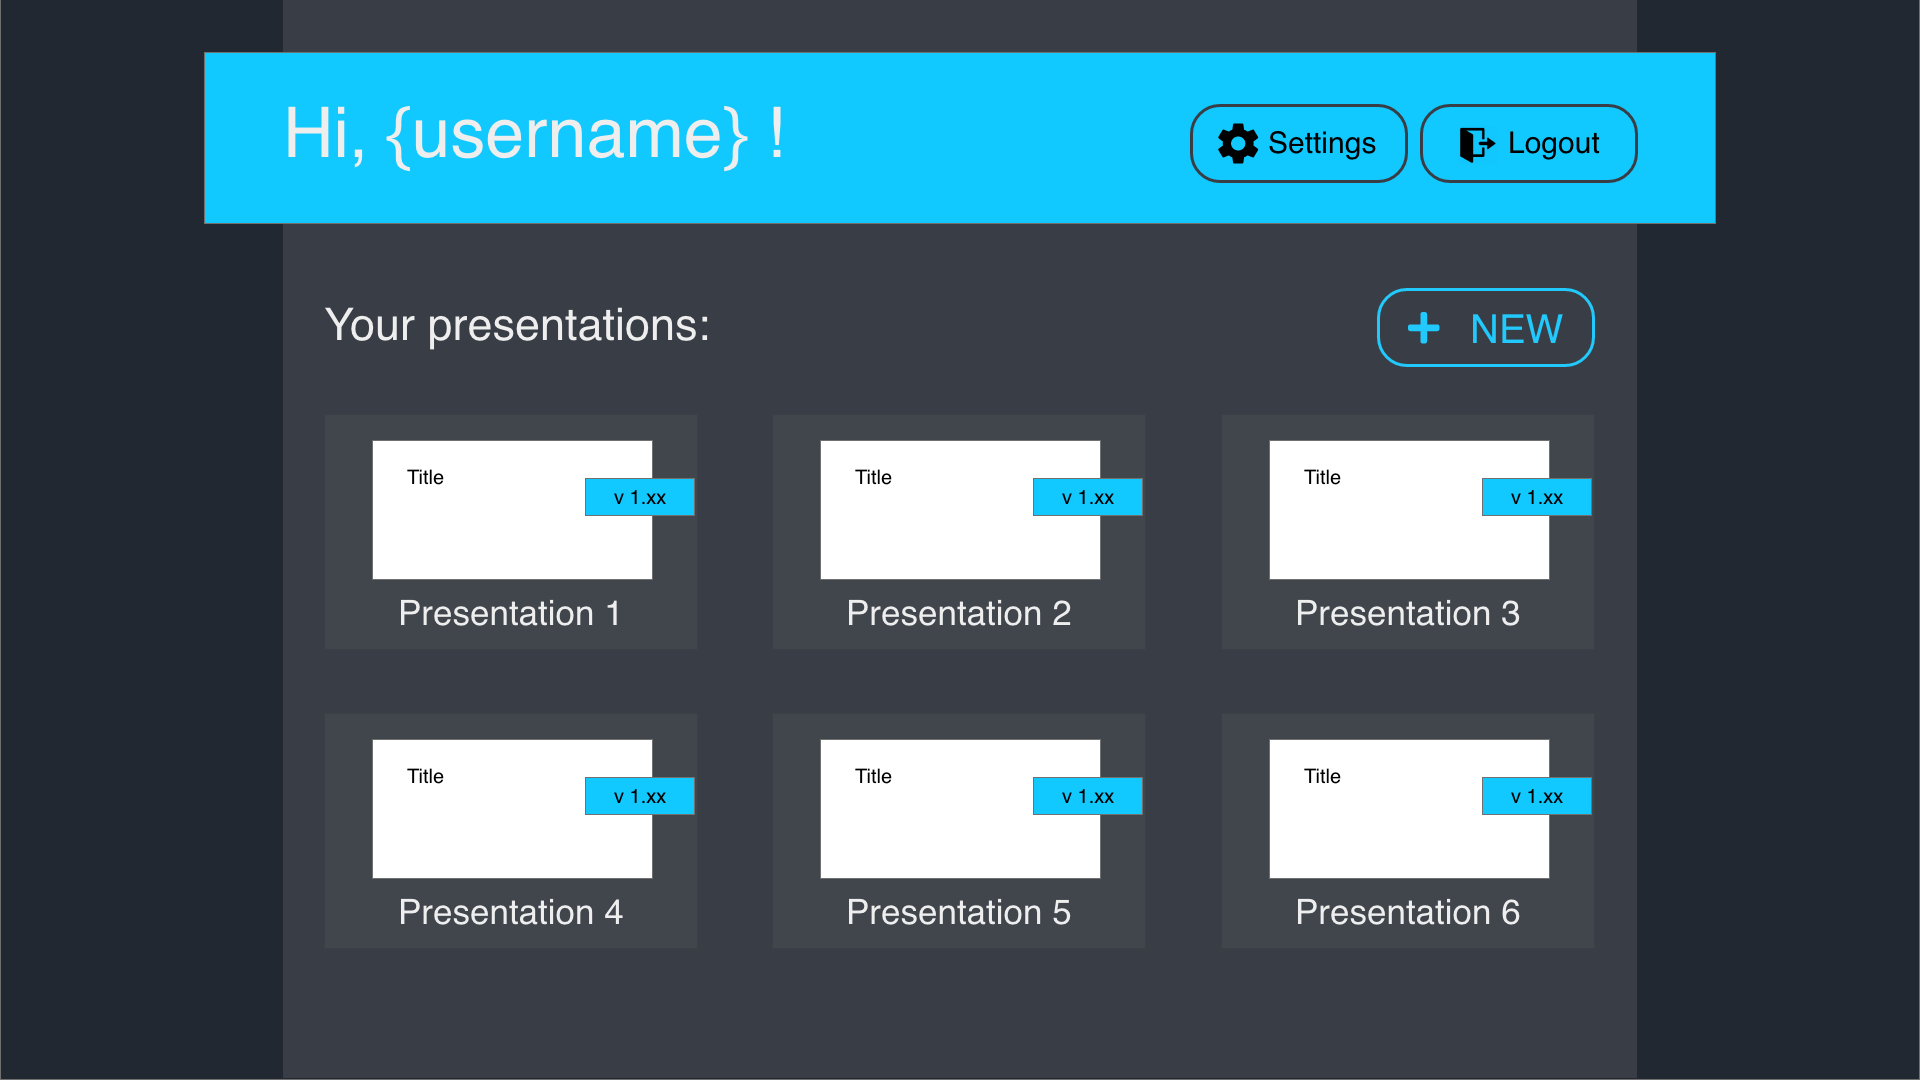
\includegraphics[scale=0.1]{obrazky/prototyp_domovska_stranka.png}
  \caption{Prototyp domovskej stránky}
  \label{pic:prototyp_domovska_stranka}
\end{minipage}%
\begin{minipage}{.5\textwidth}
  \centering
  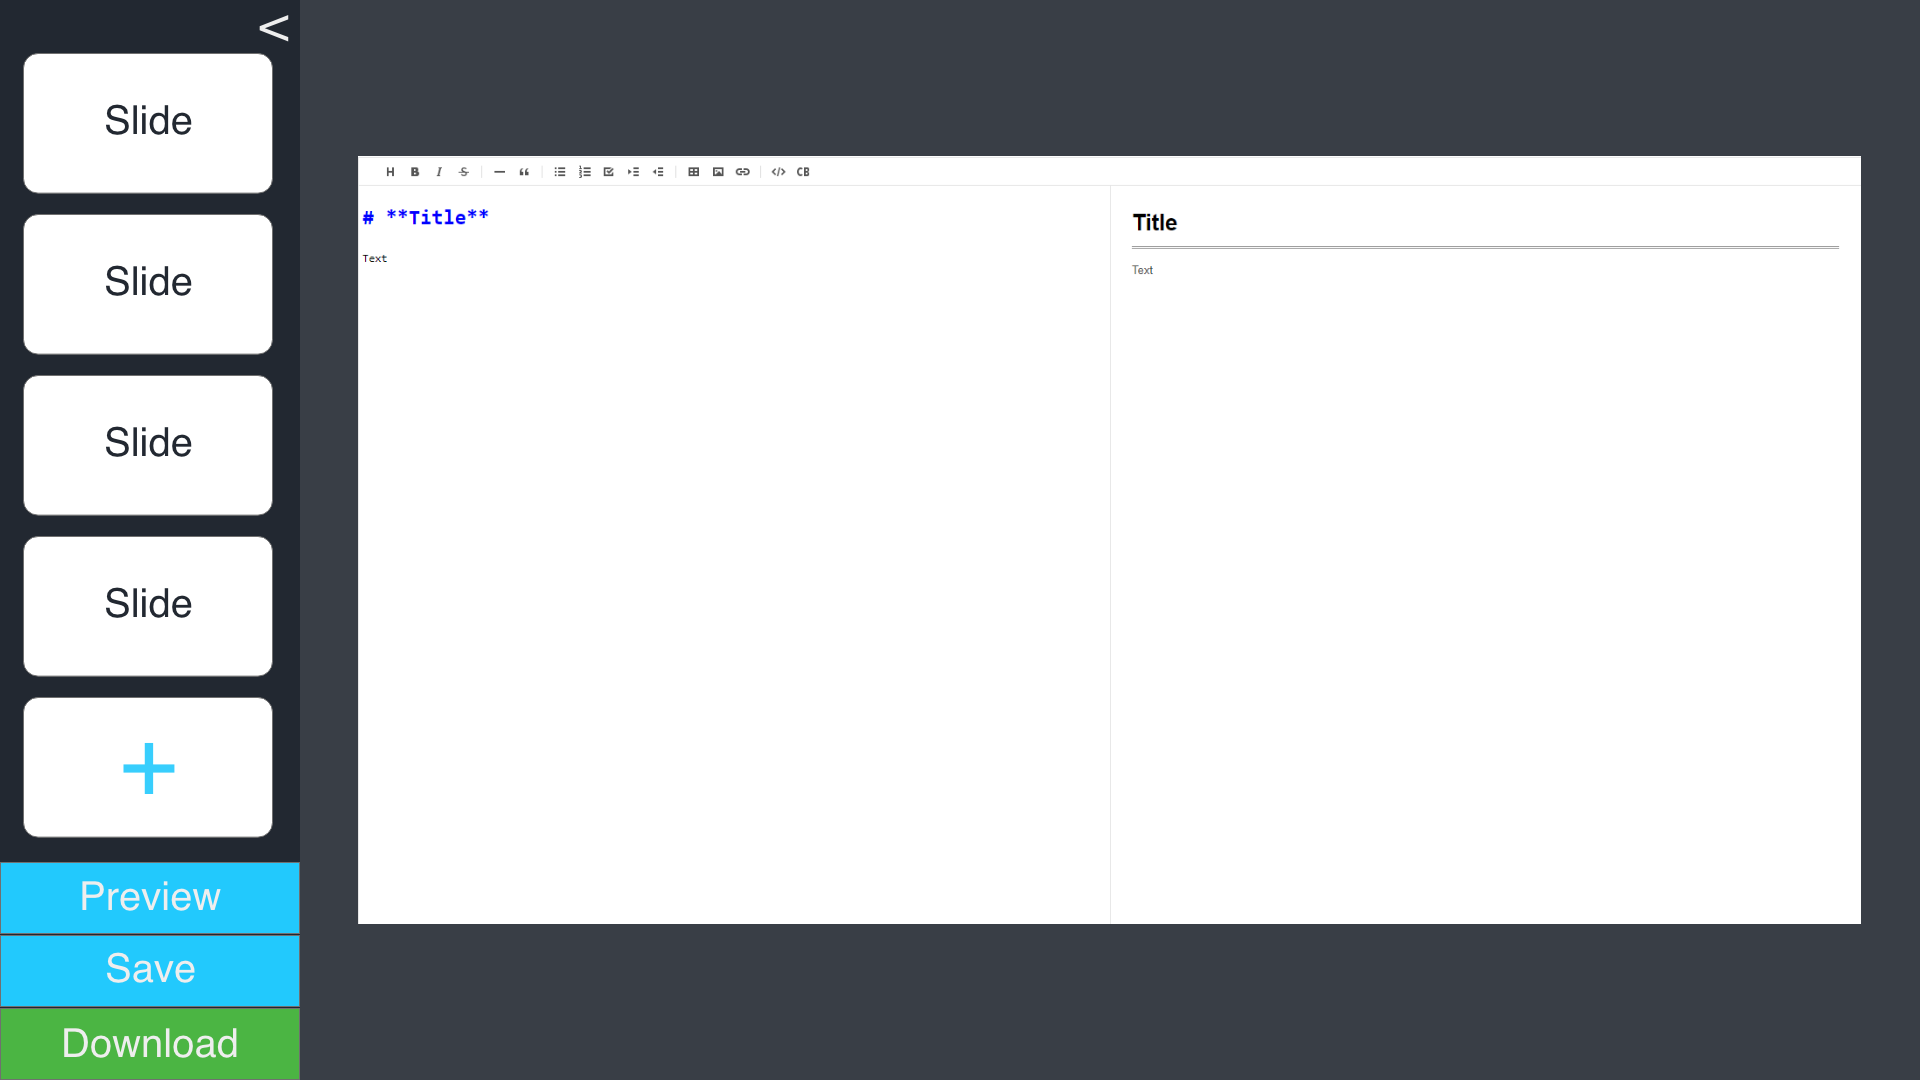
\includegraphics[scale=0.1]{obrazky/prototyp_editor.png}
  \caption{Prototyp editora}
  \label{pic:prototyp_editor}
\end{minipage}
\end{figure}

\subsection*{Autentifikačná stránka}
Autentifikačná stránka je prvá stránka, na ktorej sa užívateľ ocitne pri prvom navštívení aplikácie. Stránka obsahuje prihlasovací panel, kde je nutné zadať správny e-mail a heslo. Pri novom užívateľovi je najprv nutná registrácia cez registračný panel. Aplikácia vyžaduje iba potrebné užívateľské údaje, ako meno, e-mail a heslo.

\subsection*{Domovská stránka}
Po úspešnom prihlásení sa zobrazí domovská stránka. Domovská stránka by mala obsahovať všetky potrebné informácie pre užívateľa. Stránka je znázornená na obrázku \ref{pic:domovska_stranka}. Obsahuje tlačítko pre odhlásenie a vytvorenie novej prezentácie. Nachádza sa tu zoznam vytvorených prezentácií a tlačítka pre ich spravovanie. 

Po kliknutí na hociktorý prvok zoznamu sa zobrazí detail prezentácie. Cieľom bolo vytvoriť panel, kde sa tvorca vie dozvedieť všetko o daných verziách prezentácie bez toho, aby musel otvoriť editor. Vie si tu zvoliť danú verziu a má náhľad k jej stránkam, ktoré si môže voľne preklikať.

\begin{figure}[!hbt]
\centering
\begin{minipage}{.5\textwidth}
  \centering
  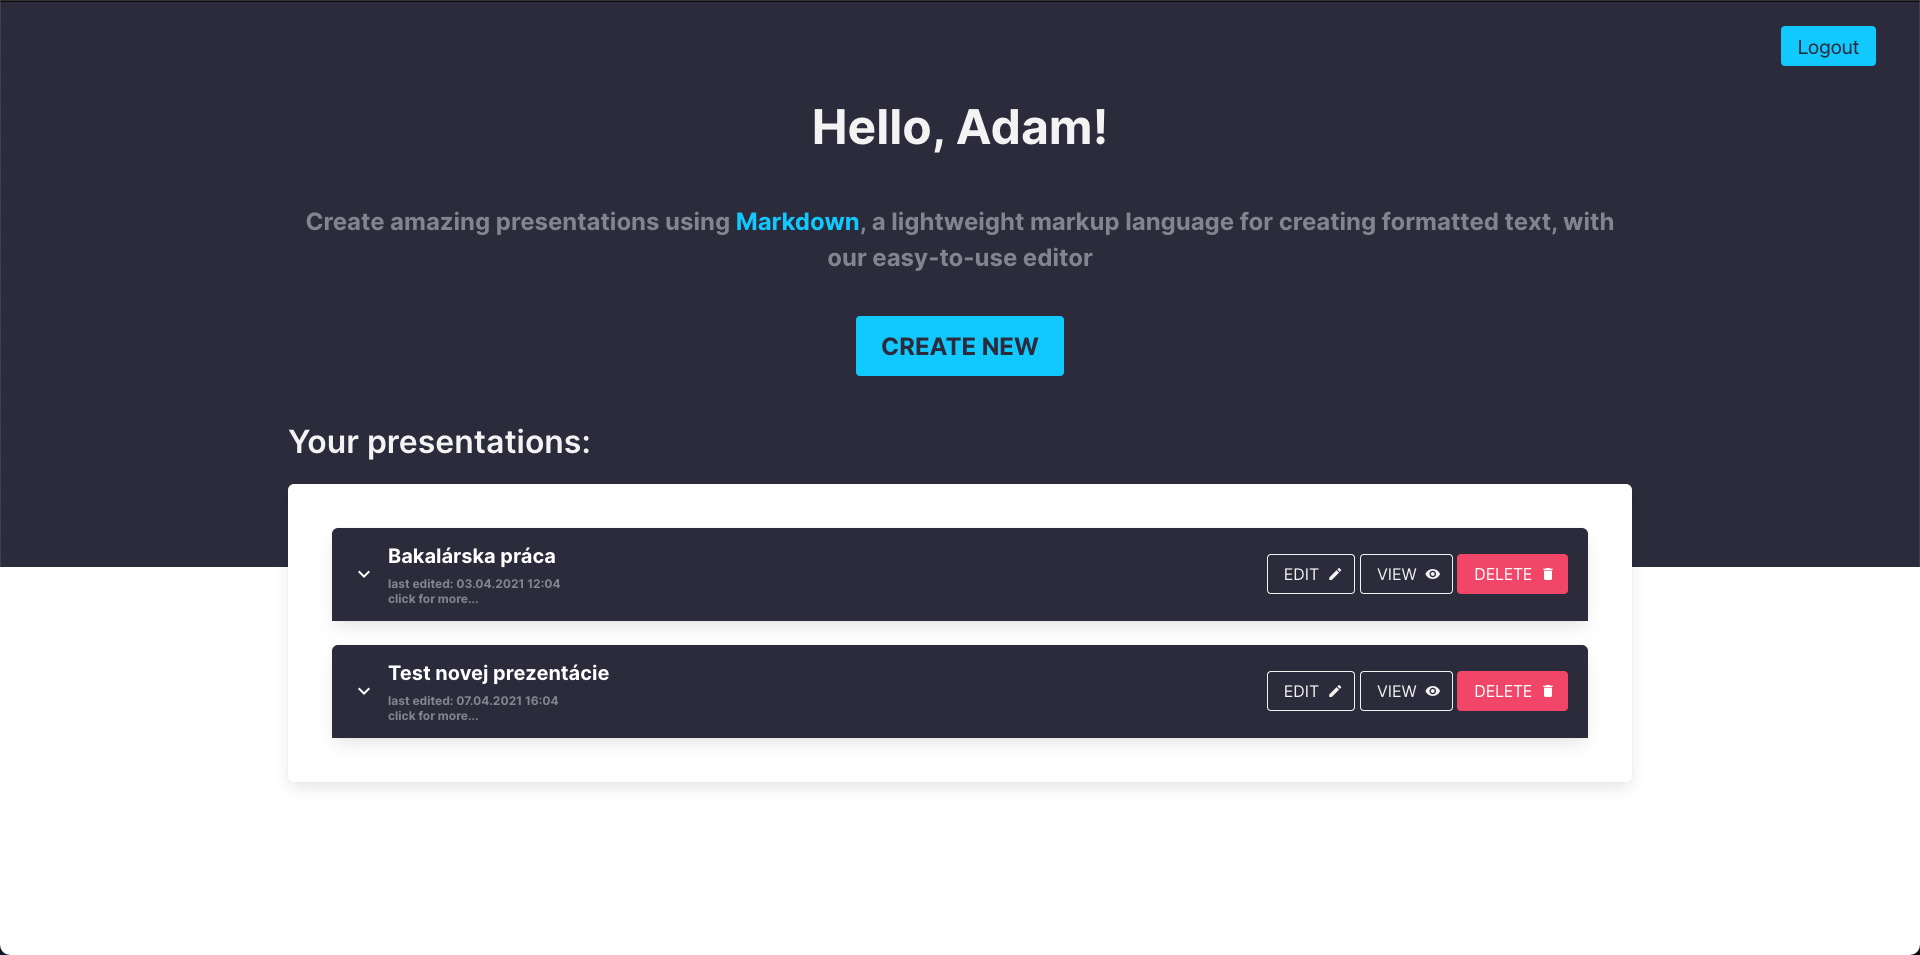
\includegraphics[scale=0.1]{obrazky/domovska_stranka.png}
  \caption{Domovská stránka}
  \label{pic:domovska_stranka}
\end{minipage}%
\begin{minipage}{.5\textwidth}
  \centering
  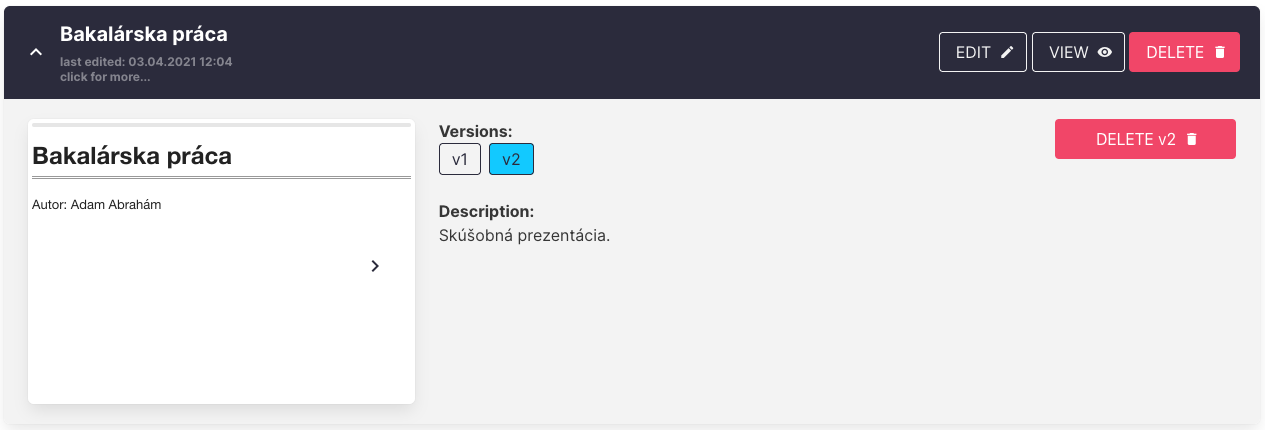
\includegraphics[scale=0.15]{obrazky/detail_prezentacie.png}
  \caption{Panel detailu prezentácie}
  \label{pic:detail_prezentacie}
\end{minipage}
\end{figure}

\subsection*{Editor}
Hlavným cieľom pri návrhu editora bolo vytvorenie stránky s čo najväčším priestorom pre písanie obsahu a náhľadom sformátovanej stránky (viď. obrázok \ref{pic:editor}). Avšak dôležité bolo správne umiestnenie nástrojov. Nástroje a ovládacie prvky by mali byť jednoducho prístupné pre tvorcu prezentácie a nemali by byť príliš schované. Pre dosiahnutie veľkého priestoru pre obsah s jednoducho prístupnými ovládacími prvkami sa navrhol vysúvací bočný panel.

Bočný panel v zavretom stave zaberá minimum priestoru na stránke a obsahuje hlavné tlačítka pre spravovanie prezentácie. Zobrazením stránok prezentácie sa bočný panel rozšíri, ako je vidieť na obrázku \ref{pic:bocny_panel}. V rozšírenom režime má tvorca prístup k zoznamu stránok, ktorý si môže zobraziť aj cez mriežkový pohľad pre jednoduchšiu orientáciu. Nad zoznamom sú dostupné tlačítka pre prácu so stránkami.

\begin{figure}[!hbt]
\centering
\begin{minipage}{.5\textwidth}
  \centering
  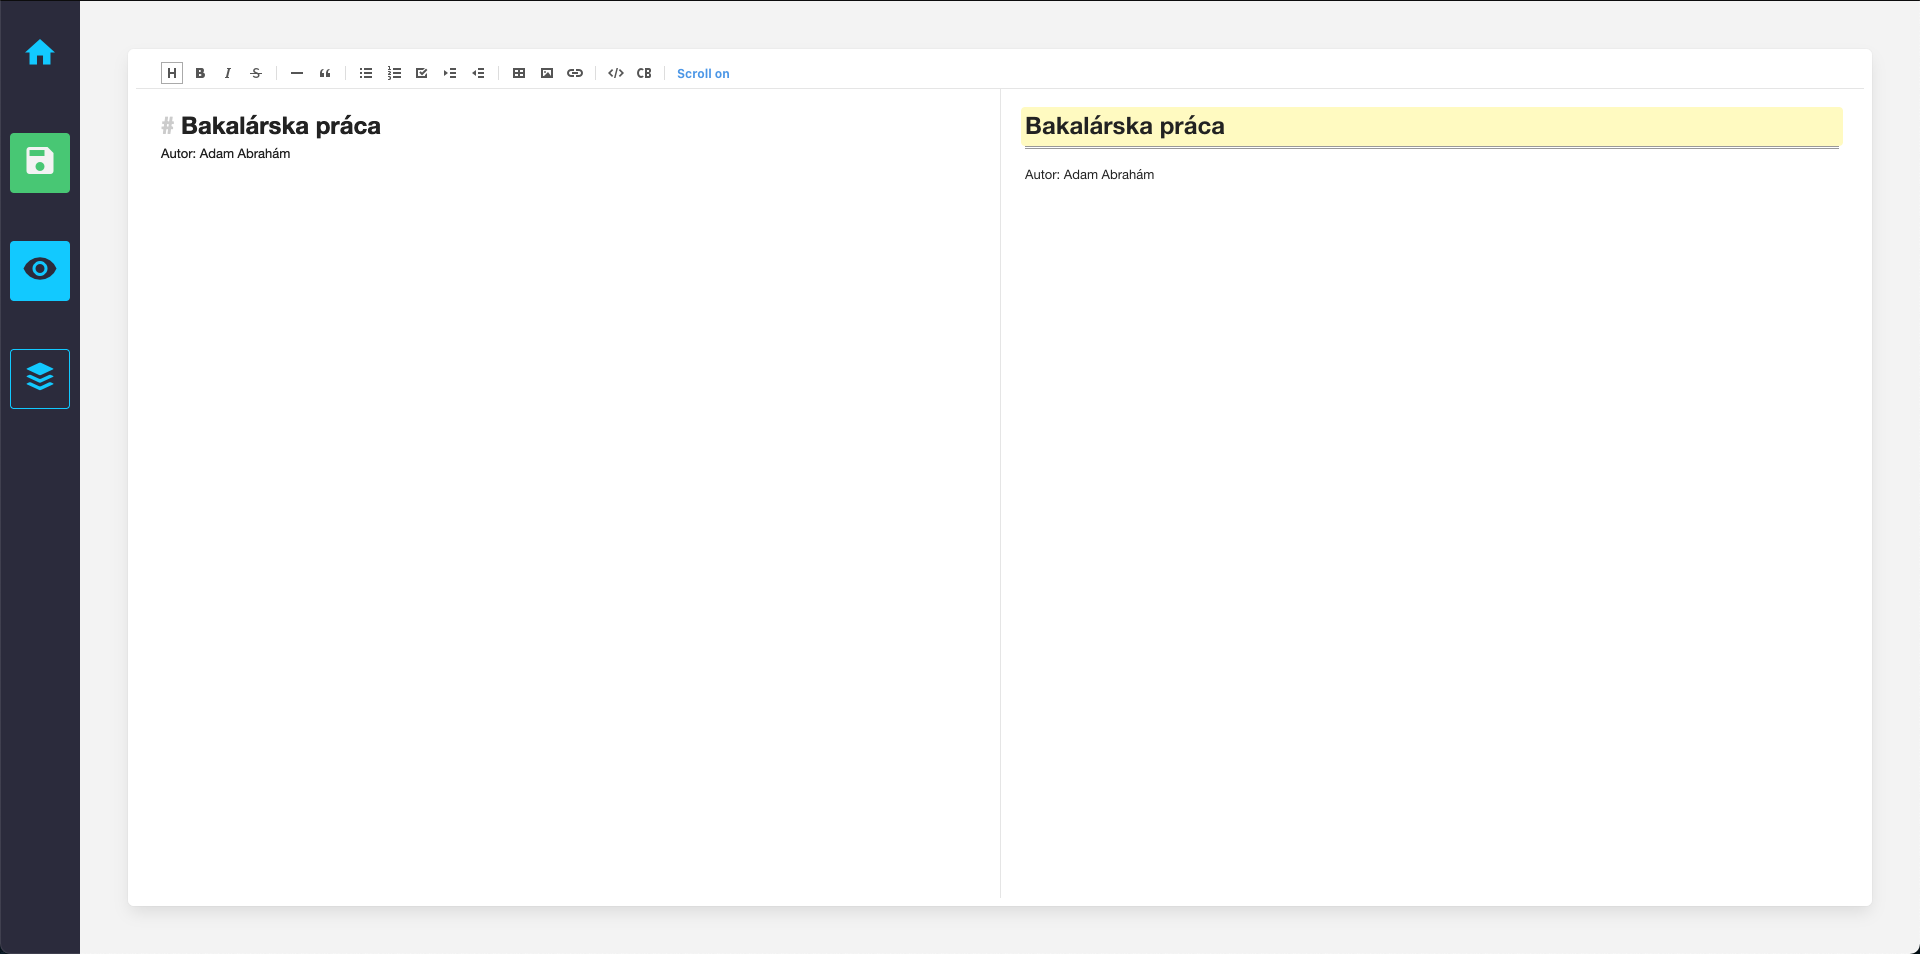
\includegraphics[scale=0.11]{obrazky/editor.png}
  \caption{Editor}
  \label{pic:editor}
\end{minipage}%
\begin{minipage}{.5\textwidth}
  \centering
  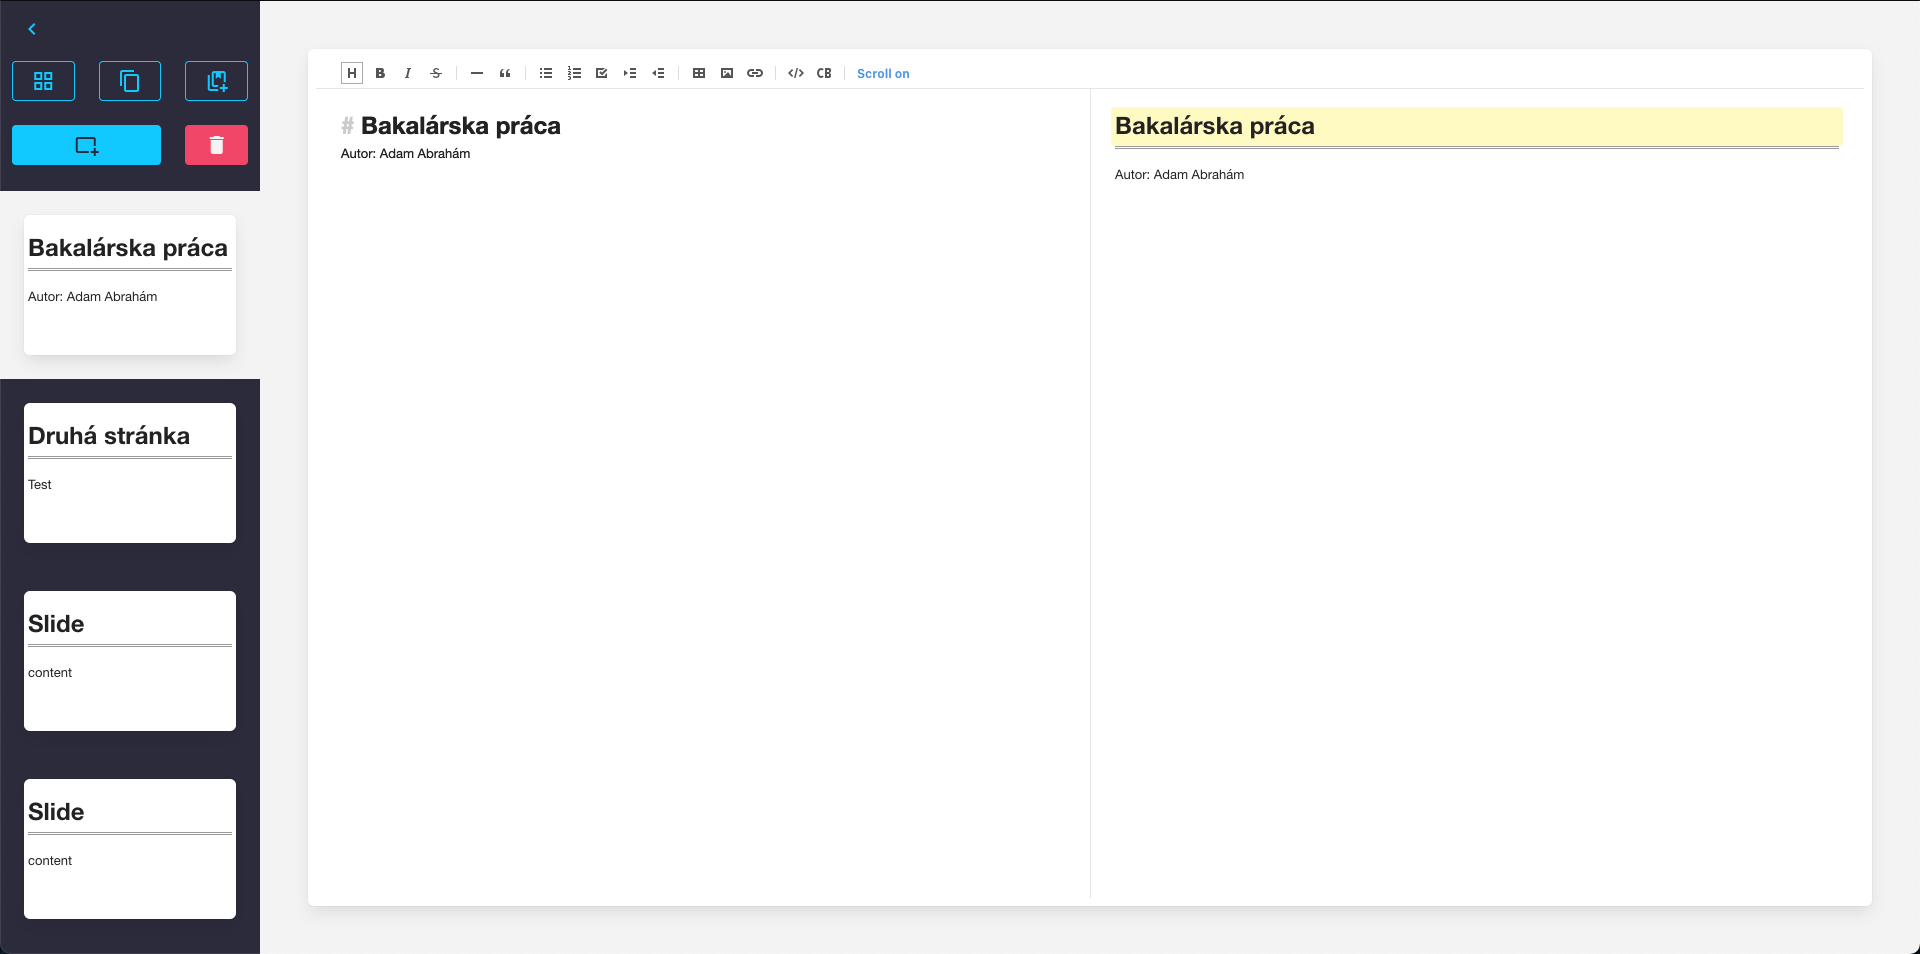
\includegraphics[scale=0.11]{obrazky/bocny_panel.png}
  \caption{Rozšírený bočný panel}
  \label{pic:bocny_panel}
\end{minipage}
\end{figure}

\subsection*{Stránka prezentácie}
Do prezentačného režimu sa užívateľ môže dostať cez domovskú stránku, ale aj cez editor. Na stránke je znázornený obsah prezentácie na celej obrazovke. Prezentácia je v tomto režime interaktívna a umožňuje prepínanie strán cez šípky klávesnice.

\section{Návrh databázy}
\label{navrhdb}
V tejto sekcii sa nachádza popis zvolených produktov pre databázu a popis uchovávanie údajov. Databáza obsahuje dve kolekcie. Nižšie sa nachádza popis oboch kolekcií a ich využitie v aplikácii. Pre jednoduchšie pochopenie, grafické znázornenie návrhu databázy je vidieť na obrázku \ref{pic:database}

\subsection*{MongoDB Atlas}
Na spravovanie a hosťovanie údajov sa používa cloudová databáza MongoDB Atlas. Pre použitie aplikácie vystačila bezplatná verzia hosťovania cez Amazon Web Services. Atlas ponúka webovú aplikáciu pre spravovanie, analýzu a zobrazenie štatistík databázy. Webová aplikácia je dostatočne zabezpečená, pre prístup k databáze je nutné pridať IP adresu do zoznamu povolených adries.  

\subsection*{Kolekcia užívateľov}
Kolekcia užívateľov uchováva dokumenty s informáciami o užívateľoch aplikácie. Nový dokument sa vytvorí pri registrácii nového užívateľa a obsahuje jeho osobné údaje, ako e-mail, krstné meno, priezvisko a heslo. Dokument naďalej obsahuje unikátny identifikátor a pole užívateľom vytvorených prezentácií. Objekty poľa uchovávajú stručné informácie o prezentácii, jej unikátny identifikátor, cez ktorý sa pristupuje ku všetkým informáciám prezentácie, dátum poslednej úpravy, názov a číslo aktuálnej verzie. K tejto kolekcii sa pristupuje po úspešnom prihlásení do aplikácie. Načítajú sa z nej údaje pre prihláseného užívateľa a informácie pre zoznam prezentácií na domovskej stránke. 

\subsection*{Kolekcia prezentácií}
Kolekcia prezentácií uchováva dokumenty s informáciami o vytvorených prezentáciách v aplikácii a o ich verziách. Dokument obsahuje unikátny identifikátor prezentácie, ktorý sa nachádza aj v zozname prezentácií užívateľa, názov prezentácie a pole verzií. Verzie v poli sú usporiadané vzostupne, od najstaršej k najnovšej. Jednotlivé objekty v tomto poli obsahujú číslo verzie, jej popis a pole obsahujúce stránky verzie. Stránky sú uchovávané v poli ako reťazce, od prvej k poslednej. Nový dokument v kolekcii sa vytvorí po uložení novej prezentácie. Nová verzia sa vytvorí v poli, keď užívateľ uloží prezentáciu ako novú verziu. Zvýšenie hodnoty čísla verzie má na starosti backend. Ku kolekcii sa pristupuje na troch miestach: na domovskej stránke pri otvorení panela detailu prezentácie, v editore pri upravovaní prezentácie a pri načítaní prezentácie v prezentačnom móde. OBRAZOK UŽIVATEĽOV !!

    \begin{figure}[!hbt]
        \centering
        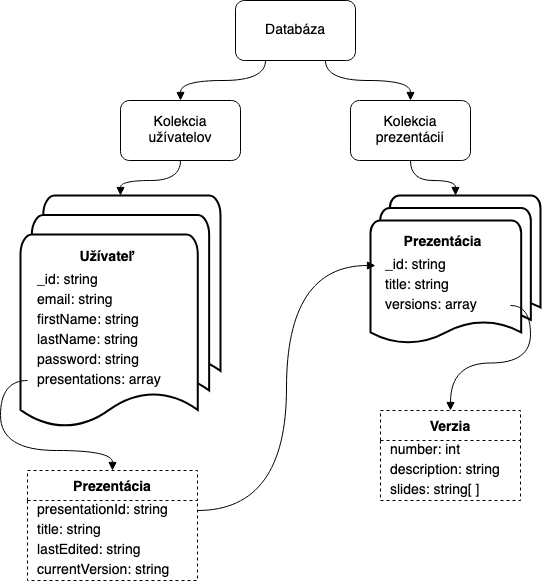
\includegraphics[scale=0.5]{obrazky/databaza.png}
        \caption{Znázornenie návrhu databáze.}
        \label{pic:database}
    \end{figure}
    
\section{Návrh backendu}
Serverová časť aplikácie prepojuje databázu s prezentačnou vrstvou. Obecne jej úlohou je sprostredkovanie komunikácie medzi nimi. Posiela HTTP odpovede na žiadosti klienta.

V tejto aplikácii má server za úlohu vytváranie, autentifikáciu, autorizáciu užívateľa, taktiež vytváranie, odstraňovanie, modifikovanie prezentácií a jeho verzií.

Návrh serverová čast sa skladá z troch hlavných vrstiev, ktoré medzi sebou komunikujú. Najnižšia je dátová vrstva, ktorá má za úlohu vytváranie mongoose schém databázy a mapovanie modelov a entít. Najvyššia vrstva je vrstva API, ktorá definuje koncové body a pristupuje k metódam repozitára. Tieto vrstvy sú prepojené vrstvou repozitára.

\subsection*{Vzor repozitára}
\label{repository}
V aplikácii je implementovaný vzor repozitára. Tento vzor pomáha v odstránení redundantného kódu. Zapúzdruje základné \texttt{CRUD} metódy nad databázou. V aplikácii sa nachádzajú dva repozitáre, repozitár užívateľa a prezentácie. K metódam repozitára sa pristupuje z API vrstvy. 

\vspace{5mm}
\dirtree{%
.1 repository.
.2 presentationRepository.
.2 userRepository.
}
\clearpage

Repozitár užívateľa obsahuje následujúce metódy:
    \begin{itemize}
        \item\texttt{getUserById} - vyhľadávanie užívateľa podľa unikátneho identifikátora
        \item\texttt{getUserByEmail} - vyhľadávanie užívateľa podľa emailu
        \item\texttt{getUserToken} - získanie autentikačného tokenu užívateľa
        \item\texttt{saveNewUser} - uloženie nového užívateľa
        \item\texttt{newPresentationSummary} - vytvorenie nového stručného popisu prezentácie
        \item\texttt{updatePresentationSummary} - aktualizácia stručného popisu prezentácie
        \item\texttt{updatePresentationSummaryCurrentVersion} - aktualizácia aktívnej verzie prezentácie
        \item\texttt{deletePresentationSummary} - odstránenie stručného popisu prezentácie
    \end{itemize}
    
\vspace{5mm}
V repozitári prezentácie sa nachádzajú metódy: 
    \begin{itemize}
        \item\texttt{getPresentation} - získanie prezentácie podľa unikátneho identifikátora
        \item\texttt{newPresentation} - vytvorenie novej prezentácie
        \item\texttt{updatePresentation} - aktualizácia prezentácie
        \item\texttt{deletePresentation} - odstránenie prezentácie
        \item\texttt{deleteVersion} - odstránenie verzie prezentácie
    \end{itemize}
    
    \subsection*{Vrstva API}
Vrstva API má za úlohu spracovávať dotazy od klienta na konkrétny koncový bod. Jednotlivé dotazy môžu obsahovať parametre v URI, takzvané query parametre, alebo parametre v tele dotazu. Pri úspešnom spracovaní dotazu API vráti HTTP odpoveď klientovi so správnym stavovým kódom \texttt{2xx}, kde čísla namiesto \texttt{x} sú doplnené podľa typu dotazu. Odpoveď môže obsahovať aj telo s obsahom. V aplikácii sa posiela obsah vo formáte JSON. Vrstva naďalej kontroluje, či je dotaz správny, či je užívateľ prihlásený a má dostačujúce oprávnenie na vykonanie dotazu, alebo či požadované dáta existujú. Pri odchytení chyby API vráti chybovú hlášku so stavovým kódom \texttt{4xx}.

\begin{table}[H]
    \centering
    \caption{Koncové body}
    \label{table:endpoints}
    \begin{tabular}{ |>{\centering\arraybackslash}m{18mm}|p{50mm}|p{70mm}|}
    \hline
    \textbf{GET} & \texttt{/api/user} & Získanie užívateľa  \\
    \hline
    \textbf{GET} & \texttt{/api/user/presentations} & Získanie prezentácií užívateľa  \\
    \hline
    \textbf{GET} & \texttt{/api/presentation} & Získanie konkrétnej prezentácie  \\
    \hline
    \textbf{POST} & \texttt{/api/auth/register} & Registrovanie užívateľa \\
    \hline
    \textbf{POST} & \texttt{/api/auth/login} & Prihlásenie užívateľa \\
    \hline
    \textbf{POST} & \texttt{/api/presentation} & Uloženie, alebo aktualizácia prezentácie  \\
    \hline
    \textbf{DELETE} & \texttt{/api/presentation} & Odstránenie prezentácie  \\
    \hline
    \textbf{DELETE} & \texttt{/api/presentation/version} & Odstránenie konkrétnej verzie prezentácie \\
    \hline
    \end{tabular}
\end{table}
